\chapter{Preambule}
\section{Probl�mes g�n�raux des transmissions de donn�es sans-fils}
Nous allons pr�senter ici les deux principaux probl�mes rencontr�s lors du
passage du signal transmis dans le canal de propagation. Ceux-ci sont li�s � la
r�ponse fr�quentielle du canal de propagation, mais ont des ph�nom�nes physiques
diff�rents.

Le premier probl�me est l�interf�rence entre symbole. Cela est d� � la
dispersion des symboles dans le temps lorsque nous en envoyons plusieurs � la suite.

L�autre probl�me est l�affaiblissement par multi-trajets, aussi appel� Fading.
Cela arrive lorsque le m�me signal � l��missions parcours des trajets diff�rents
avec r�flexions et diffractions, puis arrive sur le r�cepteur avec un d�calage
dans le temps et des variations de phases par rapport au signal re�u en trajet direct.

\section{Les signaux OFDM}

\begin{figure}[!h]
  \centering
  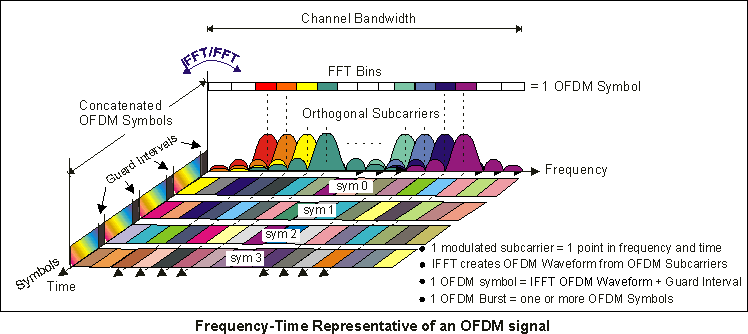
\includegraphics[width=\textwidth]{Frequence_time.png}
  \caption[Temps-Frequence]{Temps-Frequence: representation d un signal OFDM}
  \label{fig:tempsFreq}
\end{figure}

Comme nous pouvons le voir, les signaux OFDM r�sultent d�une modulation multi-porteuses. C�est-�-dire que nous r�partissons l�information sur une bande de fr�quence, autour de plusieurs porteuses de fr�quences centrales �galement r�parties. Puis, � chaque sous-fr�quences porteuses, on envoie des symboles r�partis dans le temps espac� par des intervalles de garde.



\paragraph{}